
% Default to the notebook output style

    


% Inherit from the specified cell style.




    
\documentclass{article}

    
    \usepackage{float}
    \usepackage{graphicx} % Used to insert images
    \usepackage{adjustbox} % Used to constrain images to a maximum size 
    \usepackage{color} % Allow colors to be defined
    \usepackage{enumerate} % Needed for markdown enumerations to work
    \usepackage{geometry} % Used to adjust the document margins
    \usepackage{amsmath} % Equations
    \usepackage{amssymb} % Equations
    \usepackage{eurosym} % defines \euro
    \usepackage[mathletters]{ucs} % Extended unicode (utf-8) support
    \usepackage[utf8x]{inputenc} % Allow utf-8 characters in the tex document
    \usepackage{fancyvrb} % verbatim replacement that allows latex
    \usepackage{grffile} % extends the file name processing of package graphics 
                         % to support a larger range 
    % The hyperref package gives us a pdf with properly built
    % internal navigation ('pdf bookmarks' for the table of contents,
    % internal cross-reference links, web links for URLs, etc.)
    \usepackage{hyperref}
    \usepackage{longtable} % longtable support required by pandoc >1.10
    \usepackage{booktabs}  % table support for pandoc > 1.12.2
    \usepackage{ulem} % ulem is needed to support strikethroughs (\sout)
    

    
    
    \definecolor{orange}{cmyk}{0,0.4,0.8,0.2}
    \definecolor{darkorange}{rgb}{.71,0.21,0.01}
    \definecolor{darkgreen}{rgb}{.12,.54,.11}
    \definecolor{myteal}{rgb}{.26, .44, .56}
    \definecolor{gray}{gray}{0.45}
    \definecolor{lightgray}{gray}{.95}
    \definecolor{mediumgray}{gray}{.8}
    \definecolor{inputbackground}{rgb}{.95, .95, .85}
    \definecolor{outputbackground}{rgb}{.95, .95, .95}
    \definecolor{traceback}{rgb}{1, .95, .95}
    % ansi colors
    \definecolor{red}{rgb}{.6,0,0}
    \definecolor{green}{rgb}{0,.65,0}
    \definecolor{brown}{rgb}{0.6,0.6,0}
    \definecolor{blue}{rgb}{0,.145,.698}
    \definecolor{purple}{rgb}{.698,.145,.698}
    \definecolor{cyan}{rgb}{0,.698,.698}
    \definecolor{lightgray}{gray}{0.5}
    
    % bright ansi colors
    \definecolor{darkgray}{gray}{0.25}
    \definecolor{lightred}{rgb}{1.0,0.39,0.28}
    \definecolor{lightgreen}{rgb}{0.48,0.99,0.0}
    \definecolor{lightblue}{rgb}{0.53,0.81,0.92}
    \definecolor{lightpurple}{rgb}{0.87,0.63,0.87}
    \definecolor{lightcyan}{rgb}{0.5,1.0,0.83}
    
    % commands and environments needed by pandoc snippets
    % extracted from the output of `pandoc -s`
    \providecommand{\tightlist}{%
      \setlength{\itemsep}{0pt}\setlength{\parskip}{0pt}}
    \DefineVerbatimEnvironment{Highlighting}{Verbatim}{commandchars=\\\{\}}
    % Add ',fontsize=\small' for more characters per line
    \newenvironment{Shaded}{}{}
    \newcommand{\KeywordTok}[1]{\textcolor[rgb]{0.00,0.44,0.13}{\textbf{{#1}}}}
    \newcommand{\DataTypeTok}[1]{\textcolor[rgb]{0.56,0.13,0.00}{{#1}}}
    \newcommand{\DecValTok}[1]{\textcolor[rgb]{0.25,0.63,0.44}{{#1}}}
    \newcommand{\BaseNTok}[1]{\textcolor[rgb]{0.25,0.63,0.44}{{#1}}}
    \newcommand{\FloatTok}[1]{\textcolor[rgb]{0.25,0.63,0.44}{{#1}}}
    \newcommand{\CharTok}[1]{\textcolor[rgb]{0.25,0.44,0.63}{{#1}}}
    \newcommand{\StringTok}[1]{\textcolor[rgb]{0.25,0.44,0.63}{{#1}}}
    \newcommand{\CommentTok}[1]{\textcolor[rgb]{0.38,0.63,0.69}{\textit{{#1}}}}
    \newcommand{\OtherTok}[1]{\textcolor[rgb]{0.00,0.44,0.13}{{#1}}}
    \newcommand{\AlertTok}[1]{\textcolor[rgb]{1.00,0.00,0.00}{\textbf{{#1}}}}
    \newcommand{\FunctionTok}[1]{\textcolor[rgb]{0.02,0.16,0.49}{{#1}}}
    \newcommand{\RegionMarkerTok}[1]{{#1}}
    \newcommand{\ErrorTok}[1]{\textcolor[rgb]{1.00,0.00,0.00}{\textbf{{#1}}}}
    \newcommand{\NormalTok}[1]{{#1}}
    
    % Additional commands for more recent versions of Pandoc
    \newcommand{\ConstantTok}[1]{\textcolor[rgb]{0.53,0.00,0.00}{{#1}}}
    \newcommand{\SpecialCharTok}[1]{\textcolor[rgb]{0.25,0.44,0.63}{{#1}}}
    \newcommand{\VerbatimStringTok}[1]{\textcolor[rgb]{0.25,0.44,0.63}{{#1}}}
    \newcommand{\SpecialStringTok}[1]{\textcolor[rgb]{0.73,0.40,0.53}{{#1}}}
    \newcommand{\ImportTok}[1]{{#1}}
    \newcommand{\DocumentationTok}[1]{\textcolor[rgb]{0.73,0.13,0.13}{\textit{{#1}}}}
    \newcommand{\AnnotationTok}[1]{\textcolor[rgb]{0.38,0.63,0.69}{\textbf{\textit{{#1}}}}}
    \newcommand{\CommentVarTok}[1]{\textcolor[rgb]{0.38,0.63,0.69}{\textbf{\textit{{#1}}}}}
    \newcommand{\VariableTok}[1]{\textcolor[rgb]{0.10,0.09,0.49}{{#1}}}
    \newcommand{\ControlFlowTok}[1]{\textcolor[rgb]{0.00,0.44,0.13}{\textbf{{#1}}}}
    \newcommand{\OperatorTok}[1]{\textcolor[rgb]{0.40,0.40,0.40}{{#1}}}
    \newcommand{\BuiltInTok}[1]{{#1}}
    \newcommand{\ExtensionTok}[1]{{#1}}
    \newcommand{\PreprocessorTok}[1]{\textcolor[rgb]{0.74,0.48,0.00}{{#1}}}
    \newcommand{\AttributeTok}[1]{\textcolor[rgb]{0.49,0.56,0.16}{{#1}}}
    \newcommand{\InformationTok}[1]{\textcolor[rgb]{0.38,0.63,0.69}{\textbf{\textit{{#1}}}}}
    \newcommand{\WarningTok}[1]{\textcolor[rgb]{0.38,0.63,0.69}{\textbf{\textit{{#1}}}}}
    
    
    % Define a nice break command that doesn't care if a line doesn't already
    % exist.
    \def\br{\hspace*{\fill} \\* }
    % Math Jax compatability definitions
    \def\gt{>}
    \def\lt{<}
    % Document parameters
    \title{Review of Statistical Analysis of Numerical Preclinical Radio-biological Data}
    \author{Raaz Dwivedi,  Antonio Iannopollo and Jiancong Chen}
    
    
    

    % Pygments definitions
    
\makeatletter
\def\PY@reset{\let\PY@it=\relax \let\PY@bf=\relax%
    \let\PY@ul=\relax \let\PY@tc=\relax%
    \let\PY@bc=\relax \let\PY@ff=\relax}
\def\PY@tok#1{\csname PY@tok@#1\endcsname}
\def\PY@toks#1+{\ifx\relax#1\empty\else%
    \PY@tok{#1}\expandafter\PY@toks\fi}
\def\PY@do#1{\PY@bc{\PY@tc{\PY@ul{%
    \PY@it{\PY@bf{\PY@ff{#1}}}}}}}
\def\PY#1#2{\PY@reset\PY@toks#1+\relax+\PY@do{#2}}

\expandafter\def\csname PY@tok@gd\endcsname{\def\PY@tc##1{\textcolor[rgb]{0.63,0.00,0.00}{##1}}}
\expandafter\def\csname PY@tok@gu\endcsname{\let\PY@bf=\textbf\def\PY@tc##1{\textcolor[rgb]{0.50,0.00,0.50}{##1}}}
\expandafter\def\csname PY@tok@gt\endcsname{\def\PY@tc##1{\textcolor[rgb]{0.00,0.27,0.87}{##1}}}
\expandafter\def\csname PY@tok@gs\endcsname{\let\PY@bf=\textbf}
\expandafter\def\csname PY@tok@gr\endcsname{\def\PY@tc##1{\textcolor[rgb]{1.00,0.00,0.00}{##1}}}
\expandafter\def\csname PY@tok@cm\endcsname{\let\PY@it=\textit\def\PY@tc##1{\textcolor[rgb]{0.25,0.50,0.50}{##1}}}
\expandafter\def\csname PY@tok@vg\endcsname{\def\PY@tc##1{\textcolor[rgb]{0.10,0.09,0.49}{##1}}}
\expandafter\def\csname PY@tok@vi\endcsname{\def\PY@tc##1{\textcolor[rgb]{0.10,0.09,0.49}{##1}}}
\expandafter\def\csname PY@tok@mh\endcsname{\def\PY@tc##1{\textcolor[rgb]{0.40,0.40,0.40}{##1}}}
\expandafter\def\csname PY@tok@cs\endcsname{\let\PY@it=\textit\def\PY@tc##1{\textcolor[rgb]{0.25,0.50,0.50}{##1}}}
\expandafter\def\csname PY@tok@ge\endcsname{\let\PY@it=\textit}
\expandafter\def\csname PY@tok@vc\endcsname{\def\PY@tc##1{\textcolor[rgb]{0.10,0.09,0.49}{##1}}}
\expandafter\def\csname PY@tok@il\endcsname{\def\PY@tc##1{\textcolor[rgb]{0.40,0.40,0.40}{##1}}}
\expandafter\def\csname PY@tok@go\endcsname{\def\PY@tc##1{\textcolor[rgb]{0.53,0.53,0.53}{##1}}}
\expandafter\def\csname PY@tok@cp\endcsname{\def\PY@tc##1{\textcolor[rgb]{0.74,0.48,0.00}{##1}}}
\expandafter\def\csname PY@tok@gi\endcsname{\def\PY@tc##1{\textcolor[rgb]{0.00,0.63,0.00}{##1}}}
\expandafter\def\csname PY@tok@gh\endcsname{\let\PY@bf=\textbf\def\PY@tc##1{\textcolor[rgb]{0.00,0.00,0.50}{##1}}}
\expandafter\def\csname PY@tok@ni\endcsname{\let\PY@bf=\textbf\def\PY@tc##1{\textcolor[rgb]{0.60,0.60,0.60}{##1}}}
\expandafter\def\csname PY@tok@nl\endcsname{\def\PY@tc##1{\textcolor[rgb]{0.63,0.63,0.00}{##1}}}
\expandafter\def\csname PY@tok@nn\endcsname{\let\PY@bf=\textbf\def\PY@tc##1{\textcolor[rgb]{0.00,0.00,1.00}{##1}}}
\expandafter\def\csname PY@tok@no\endcsname{\def\PY@tc##1{\textcolor[rgb]{0.53,0.00,0.00}{##1}}}
\expandafter\def\csname PY@tok@na\endcsname{\def\PY@tc##1{\textcolor[rgb]{0.49,0.56,0.16}{##1}}}
\expandafter\def\csname PY@tok@nb\endcsname{\def\PY@tc##1{\textcolor[rgb]{0.00,0.50,0.00}{##1}}}
\expandafter\def\csname PY@tok@nc\endcsname{\let\PY@bf=\textbf\def\PY@tc##1{\textcolor[rgb]{0.00,0.00,1.00}{##1}}}
\expandafter\def\csname PY@tok@nd\endcsname{\def\PY@tc##1{\textcolor[rgb]{0.67,0.13,1.00}{##1}}}
\expandafter\def\csname PY@tok@ne\endcsname{\let\PY@bf=\textbf\def\PY@tc##1{\textcolor[rgb]{0.82,0.25,0.23}{##1}}}
\expandafter\def\csname PY@tok@nf\endcsname{\def\PY@tc##1{\textcolor[rgb]{0.00,0.00,1.00}{##1}}}
\expandafter\def\csname PY@tok@si\endcsname{\let\PY@bf=\textbf\def\PY@tc##1{\textcolor[rgb]{0.73,0.40,0.53}{##1}}}
\expandafter\def\csname PY@tok@s2\endcsname{\def\PY@tc##1{\textcolor[rgb]{0.73,0.13,0.13}{##1}}}
\expandafter\def\csname PY@tok@nt\endcsname{\let\PY@bf=\textbf\def\PY@tc##1{\textcolor[rgb]{0.00,0.50,0.00}{##1}}}
\expandafter\def\csname PY@tok@nv\endcsname{\def\PY@tc##1{\textcolor[rgb]{0.10,0.09,0.49}{##1}}}
\expandafter\def\csname PY@tok@s1\endcsname{\def\PY@tc##1{\textcolor[rgb]{0.73,0.13,0.13}{##1}}}
\expandafter\def\csname PY@tok@ch\endcsname{\let\PY@it=\textit\def\PY@tc##1{\textcolor[rgb]{0.25,0.50,0.50}{##1}}}
\expandafter\def\csname PY@tok@m\endcsname{\def\PY@tc##1{\textcolor[rgb]{0.40,0.40,0.40}{##1}}}
\expandafter\def\csname PY@tok@gp\endcsname{\let\PY@bf=\textbf\def\PY@tc##1{\textcolor[rgb]{0.00,0.00,0.50}{##1}}}
\expandafter\def\csname PY@tok@sh\endcsname{\def\PY@tc##1{\textcolor[rgb]{0.73,0.13,0.13}{##1}}}
\expandafter\def\csname PY@tok@ow\endcsname{\let\PY@bf=\textbf\def\PY@tc##1{\textcolor[rgb]{0.67,0.13,1.00}{##1}}}
\expandafter\def\csname PY@tok@sx\endcsname{\def\PY@tc##1{\textcolor[rgb]{0.00,0.50,0.00}{##1}}}
\expandafter\def\csname PY@tok@bp\endcsname{\def\PY@tc##1{\textcolor[rgb]{0.00,0.50,0.00}{##1}}}
\expandafter\def\csname PY@tok@c1\endcsname{\let\PY@it=\textit\def\PY@tc##1{\textcolor[rgb]{0.25,0.50,0.50}{##1}}}
\expandafter\def\csname PY@tok@o\endcsname{\def\PY@tc##1{\textcolor[rgb]{0.40,0.40,0.40}{##1}}}
\expandafter\def\csname PY@tok@kc\endcsname{\let\PY@bf=\textbf\def\PY@tc##1{\textcolor[rgb]{0.00,0.50,0.00}{##1}}}
\expandafter\def\csname PY@tok@c\endcsname{\let\PY@it=\textit\def\PY@tc##1{\textcolor[rgb]{0.25,0.50,0.50}{##1}}}
\expandafter\def\csname PY@tok@mf\endcsname{\def\PY@tc##1{\textcolor[rgb]{0.40,0.40,0.40}{##1}}}
\expandafter\def\csname PY@tok@err\endcsname{\def\PY@bc##1{\setlength{\fboxsep}{0pt}\fcolorbox[rgb]{1.00,0.00,0.00}{1,1,1}{\strut ##1}}}
\expandafter\def\csname PY@tok@mb\endcsname{\def\PY@tc##1{\textcolor[rgb]{0.40,0.40,0.40}{##1}}}
\expandafter\def\csname PY@tok@ss\endcsname{\def\PY@tc##1{\textcolor[rgb]{0.10,0.09,0.49}{##1}}}
\expandafter\def\csname PY@tok@sr\endcsname{\def\PY@tc##1{\textcolor[rgb]{0.73,0.40,0.53}{##1}}}
\expandafter\def\csname PY@tok@mo\endcsname{\def\PY@tc##1{\textcolor[rgb]{0.40,0.40,0.40}{##1}}}
\expandafter\def\csname PY@tok@kd\endcsname{\let\PY@bf=\textbf\def\PY@tc##1{\textcolor[rgb]{0.00,0.50,0.00}{##1}}}
\expandafter\def\csname PY@tok@mi\endcsname{\def\PY@tc##1{\textcolor[rgb]{0.40,0.40,0.40}{##1}}}
\expandafter\def\csname PY@tok@kn\endcsname{\let\PY@bf=\textbf\def\PY@tc##1{\textcolor[rgb]{0.00,0.50,0.00}{##1}}}
\expandafter\def\csname PY@tok@cpf\endcsname{\let\PY@it=\textit\def\PY@tc##1{\textcolor[rgb]{0.25,0.50,0.50}{##1}}}
\expandafter\def\csname PY@tok@kr\endcsname{\let\PY@bf=\textbf\def\PY@tc##1{\textcolor[rgb]{0.00,0.50,0.00}{##1}}}
\expandafter\def\csname PY@tok@s\endcsname{\def\PY@tc##1{\textcolor[rgb]{0.73,0.13,0.13}{##1}}}
\expandafter\def\csname PY@tok@kp\endcsname{\def\PY@tc##1{\textcolor[rgb]{0.00,0.50,0.00}{##1}}}
\expandafter\def\csname PY@tok@w\endcsname{\def\PY@tc##1{\textcolor[rgb]{0.73,0.73,0.73}{##1}}}
\expandafter\def\csname PY@tok@kt\endcsname{\def\PY@tc##1{\textcolor[rgb]{0.69,0.00,0.25}{##1}}}
\expandafter\def\csname PY@tok@sc\endcsname{\def\PY@tc##1{\textcolor[rgb]{0.73,0.13,0.13}{##1}}}
\expandafter\def\csname PY@tok@sb\endcsname{\def\PY@tc##1{\textcolor[rgb]{0.73,0.13,0.13}{##1}}}
\expandafter\def\csname PY@tok@k\endcsname{\let\PY@bf=\textbf\def\PY@tc##1{\textcolor[rgb]{0.00,0.50,0.00}{##1}}}
\expandafter\def\csname PY@tok@se\endcsname{\let\PY@bf=\textbf\def\PY@tc##1{\textcolor[rgb]{0.73,0.40,0.13}{##1}}}
\expandafter\def\csname PY@tok@sd\endcsname{\let\PY@it=\textit\def\PY@tc##1{\textcolor[rgb]{0.73,0.13,0.13}{##1}}}

\def\PYZbs{\char`\\}
\def\PYZus{\char`\_}
\def\PYZob{\char`\{}
\def\PYZcb{\char`\}}
\def\PYZca{\char`\^}
\def\PYZam{\char`\&}
\def\PYZlt{\char`\<}
\def\PYZgt{\char`\>}
\def\PYZsh{\char`\#}
\def\PYZpc{\char`\%}
\def\PYZdl{\char`\$}
\def\PYZhy{\char`\-}
\def\PYZsq{\char`\'}
\def\PYZdq{\char`\"}
\def\PYZti{\char`\~}
% for compatibility with earlier versions
\def\PYZat{@}
\def\PYZlb{[}
\def\PYZrb{]}
\makeatother


    % Exact colors from NB
    \definecolor{incolor}{rgb}{0.0, 0.0, 0.5}
    \definecolor{outcolor}{rgb}{0.545, 0.0, 0.0}




    % Prevent overflowing lines due to hard-to-break entities
    \sloppy
    % Setup hyperref package
    \hypersetup{
      breaklinks=true,  % so long urls are correctly broken across lines
      colorlinks=true,
      urlcolor=blue,
      linkcolor=black,
      citecolor=darkgreen,
      }
    % Slightly bigger margins than the latex defaults

    \geometry{verbose,tmargin=1in,bmargin=1in,lmargin=1in,rmargin=1in}



    \begin{document}


    \maketitle



\begin{abstract}
This review reproduces tests and results
presented by Pitt and Hill and discusses some other non-parametric techniques, such as Permutation Tests, which allow to analyze data with less restrictive assumptions. 
The focus of this review is on the statistical methodology more than the underlying biological aspects and assumptions of the original work, which are not discussed.
Although not expert in statistical methods for fraud detection, we do believe that permutation tests are promising in this context, as demonstrated by the results presented here. 
This review has been developed as a term
project for a Graduate Level Course on Statistical Models at University of California Berkeley, by graduate
students from EECS and Civil\&Environmental Engineering departments.
\end{abstract}

\section{Introduction} % (fold)
\label{sec:introduction}

% section introduction (end)

We review the paper in the spirit of promoting reproducibility of research and attempt to replicate the authors' work. We also discuss other methods to identify anomalies, and present results based on our analysis using Permutation Tests. Permutation tests are consistent with the aim of the paper--providing simple tools to detect anomalies--and validate the results in the paper, leading to the same conclusions.

Before diving into technical details, we offer a minor suggestion: we would have found the paper easier to read if the sections and subsections had been numbered.
The review is organized as follows.
In Section~\ref{reproducibility-of-results} we replicate authors' work and results. 
In Section~\ref{our-analysis}, we analyze weaknesses of the approach followed in the paper and propose additional techniques to consolidate results. 
We finally draw our conclusions in Section~\ref{conclusion}.

\subsection{Problem Set Up}\label{problem-set-up}

The paper begins by voicing a growing concern towards ``Scientific fraud
and Plagiarism'' in the scientific community and is successful in
sending a strong message. The authors present some statistical figures and point the existence of easy statistical tools to detect fabricated data and ignorance about the tools. 

The authors examine patterns in radio-biological data. They find that data reported by one of 10 researchers, the "RTS," is suspicious. 
They perform three different
tests to validate their suspicion and also validate their tests and
assumptions by looking at the data obtained from three other sources.

Each researcher made two types of triplicate measurements - colony counts and Coulter counts.  
The authors suspect that the RTS fabricated data triples to get the mean s/he desired in each triple by setting one observation equal to the desired mean and the other two equal distances above and below that value. This would result in triples that contain the (rounded) mean as one of the values.

The methodological contribution of the paper is “bounds and estimates for the probability that a given set of n such triplicates contains k or more triples which contain their own mean” when each of the $n$ triples is independent and identically distributed (IID) Poisson, and triples are independent of each other. (Different triples may have different Poisson rates.)
For this Poisson model, the chance that the RTS's data would contain so many triples that include their mean is astronomically low.
They also apply more common tests for anomalous data, based on statistics such as the frequency of the terminal digit and the frequency with which the last two digits are equal.

However, some of the questions that were slightly untouched upon are discussed below:

\begin{itemize}
\item
  The authors write, “Having observed what appeared to us to be an unusual frequency of triples in RTS data containing a value close to their mean, we used R to calculate the mid-ratios for all of the colony data triples that were available to us.” This suggests that the same data--and the same feature of the data--that raised their suspicions about the RTS was the data used to test whether the RTS's data were anomalous on the basis of that feature. If so, then the nominal p-values are likely to be misleadingly small.
\item
  Most of the tests compare the RTS data to what would be expected for a model of the observations, then validate the test by comparing data pooled for the other researchers to the model. Pooling the data in this way may hide anomalies in the other researchers' data. Permutation tests allow the data for the RTS to be compared to the data for the other researchers (and to compare each researcher's data with that of the group) without positing a model for how the data were generated. On the other hand, the bulk of the data available are for the RTS, so to reject the hypothesis that another researcher's data looks like a random sample from the pooled data--if it includes the RTS's data--primarily shows that that researcher's data is not like that of the RTS, not that they are suspicious. See section~\ref{our-analysis} of this review for more discussion.
\end{itemize}

    \section{Reproducibility of Results}\label{reproducibility-of-results}

This section discusses our efforts to replicate the analyses in the paper. 
After some trial and error and fine tuning we were able to replicate most of
their results, obtaining similar results in the other cases. All our
material and code is available on \hyperlink{https://github.com/ianno/stat215a_project1}{github}[github.com/ianno/stat215a\_project1]. We first discuss specifics about the replication and then comment about the tests and methods involved.


    \subsection{Mid-Ratio Analysis}\label{mid-ratio-analysis}

The authors first consider the mid-ratio of th samples, which is defined for a triplet \((a, b, c), a<b<c\) as
\(\frac{b-a}{c-a}\), and show that the histogram of RTS' samples concentrates
abnormally around the \(0.4-0.6\) range, compared to the samples taken by all the other lab members. 
We tried to reproduce the histogram using both numpy (python) and Matlab, but it
looked very different from the one on the paper. 
To get a closer representation, we had to tweak the default histogram plot function (every bin had to include its right bound). 
The histogram, however, still had some differences.
For instance, 
in the paper, the chance of obtaining a mid-ratio of
0.4-0.5 is almost 50\%, while in our case is 44\%.
Additionally, we could not find any information about the data cleaning and pre-processing procedures used by the authors.
After cleaning the data, for instance, we got 1360 usable RTS samples out of 1361, while
the authors only used 1343.
A similar situation occurred for the number of samples of the other lab members.
Although not being a major issue, this has had a negative impact on our analyses since we have not been able to reproduce \textit{exactly} all of the results.


    \subsection{Probability Model for Sample Triples}\label{probability-model}
TODO: is this correct?check

The authors modeled each triple of observations as three i.i.d. Poisson random variables with mean $\lambda$ (which could be different for each triple).
The occurrence of the (rounded) mean of each triple as one of its value is then modeled as a Bernoulli random variable parameterized according to a certain $\lambda$ (tabulated in Table 1).
The author provided also an analytical description of this model, which in our opinion is reasonable, in the Appendix.
We have been able to replicate Table 1 according to the given analytical model, although we got some numerical issues for large $\lambda$ (which, however, did not impact the rest of our analysis).
With this information, proving the correctness of the hypothesis test 1 in the paper was straightforward.

TODO we missed coverage of hypothesis 1?
    \subsubsection{Using $\lambda$ to obtain
p-values}\label{using-lambda-to-obtain-p-values}
TODO: this needs major revision.
it does not say what they did. and why our implementation doesn't work for larger values. Also, we should cite the literature reference we make.
Also, do we miss hypothesis test 3?

In this section, the researchers used their probability model calculations to compute the chance of observing the data. While replicating,
it worked fine for us with the colony data as the mean of the counts $<100$, and we were able to replicate their computations to minor errors. However, when we conducted the same experiments for Coulter data, due to the limitation of our implementations, we could barely come up with a reasonable probability value as the mean value of counts were a lot larger, and thus we could not replicate the values for the Coulter. We tried a regression based on the statement from the
literature that when $\lambda = 100$ we use probability $<0.14$, and for $\lambda = 2000$ we use probability $= 0.032$. However the take away message is hardly unaffected, and these section were not the focus of our review. For completeness we mention the interpolated probabilities for Coulter Data used for computing statistics as in Table 2 of the original paper:

\begin{figure}[H]
\centering
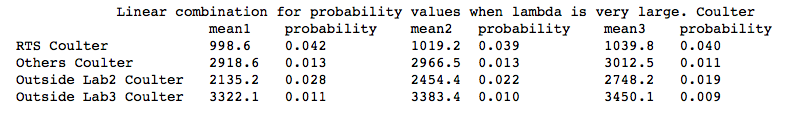
\includegraphics[width=0.9\linewidth]{images/Lambda_Coulter.png}
\caption{Approximate $p$-values for Coulter Data}
\end{figure}

\begin{figure}[H]
\centering
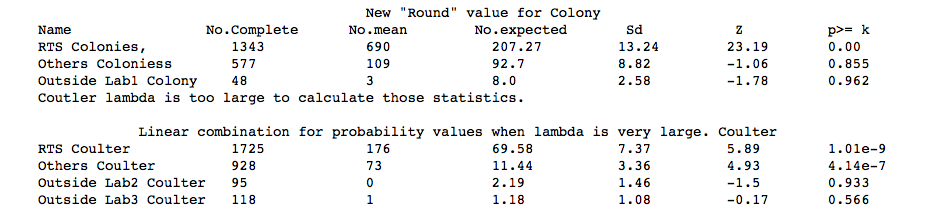
\includegraphics[width=0.9\linewidth]{images/HT_Stat_values.png}
\caption{Approximate Replication of Table 2}
\end{figure}

    \subsection{Digits Analysis}\label{digits-analysis}

To find additional confirmations on the suspicion of fabricated data, the
authors perform two additional tests, namely \textit{terminal
digit analysis} and \textit{pair of equal terminal digits analysis}. Both
such analyses are based on the intuitive observation (also supported by a reference in the paper) that the least significant digit of a sample is, in general, not very informative, i.e.~it is reasonable to expect it to be uniformly distributed random variable.



\subsubsection{Terminal digit analysis}\label{terminal-digit-analysis}

The assumption behind this test is that for experiments including
counts, the last digit of a measure represented by a large number
($>100$) can be expected to be uniformly distributed. On the
other hand, fabricated data often fail to show such peculiar property.
The authors use the chi-square test for goodness of fit to demonstrate
the fraudulent nature of RTS' samples. Our results are very similar to
the ones in the paper, although not identical.
We identified in the small difference in number of data points used, as pointed in Section~\ref{mid-ratio-analysis}, the root of this discrepancy.

\subsubsection{Equal digits analysis}\label{equal-digits-analysis}

This test follows from the same assumptions made in Section~\ref{terminal-digit-analysis}.
The claim is that in case of genuine data, one should see a pair of equal terminal digits only in 1/10 of the samples. 
Also in this case, to make sure to consider only insignificant digits, the
authors limit their analysis to large numbers (>100). 
For this experiment, however,
the authors fail to state what kind of test they have performed (we
assume chi-square test for goodness again) and how the data was
pre-processed. 
This assumption led us to obtain similar, but not identical results.



\subsubsection{Discussion on Methodology}\label{discussion-of-assumptions}
Here are a few general comments on the methodology adopted by the authors:
\begin{itemize}
    \item We felt that the justification for the Poisson assumption for the triplet data was not very strong. 
    And the applicability of the model to the data was also not exhaustively discussed. 
    \item Although one can argue that the parameters fitted to the suspected data should not be used to test the validity of the data, we agree with the authors that such a practice only lowers the chances of the suspicion, and gives the person in question the benefit of doubt.
    \item The authors provide a reference for the uniformity of last insignificant digit to a work \cite{mosimann2002terminal}, but fail in explaining why such framework can safely be applied in the context they analyze. 
    For instance, there
    might be some characteristics of the underlying biological process which
    prevent the last digits to be uniformly distributed. 
    An attempt to
    clarify and justify this choice in the current setting would have been
    beneficial. 
    \item The authors include additional data, provided by three
    external sources (two for Coulter and one for colony counts) which suffered from relatively very low number of data points.
    Although the authors comment on the size of these additional datasets
    in the Discussion section, we still believe that, in the current
    setting, these additional samples do not help them in making a stronger
    case, but instead can be misleading and definitely added to our confusion.
    \item We reiterate that treating all the other lab
    investigators as a single pool and singling out RTS is not sufficient, since uniformity
    of the pool does not necessarily imply a similar property for each contributors. 

\end{itemize}



    \section{Proposed Analysis}\label{our-analysis}

We claim that the approach followed in the paper is flawed by the initial suspicion towards RTS, for which the authors do not provide clear support.
Additionally, the choice of grouping all the other lab members in a single group \textit{against} RTS seems unfair in principle.
The main concern is that other members in the lab could have collected data similar to those of RTS --maybe because of particular characteristics of the experiments, or for common malpractice-- which is not evident when all the observations are grouped in a single pool.

Moreover, how do we single out the
malicious researcher if we don't know \textit{a priori} who he/she is? 
If we decide to use the histogram of sample mid-ratios as the first test, 
then a simple
way would be to plot histograms for all researchers, \textit{individually} and as a group, and look for anomalous patterns
across all these plots. 
Such an experiment, illustrated in Figure~\ref{fig:individuals}, gives very
interesting results and also raises an important questions about the approach followed in the paper:
\begin{figure}[H]
\label{fig:individuals}
\centering
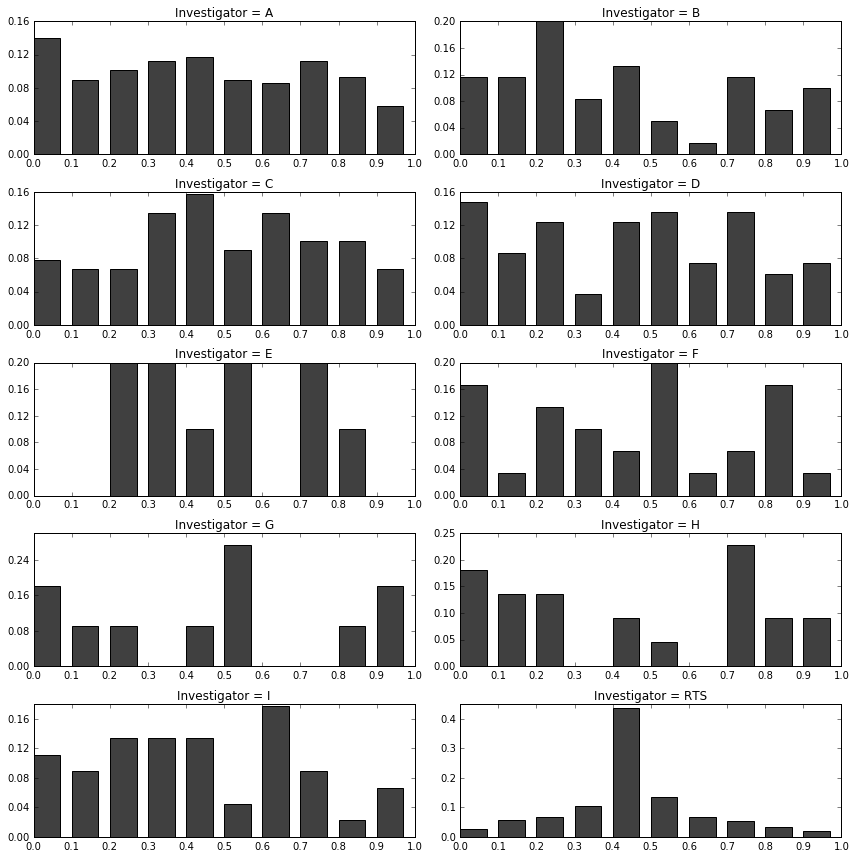
\includegraphics[width=0.8\linewidth]{images/new_mid_ratio.png}
\caption{Individual Histograms for the Colony Data}
\end{figure}

\begin{itemize}
\item
  The histograms for researchers with labels ``B, C, E, F, G, H, I'' do not
  seem to be close to uniform as well. 
  In particular, ``B'' and ``C''
  look very unlikely to represent an underlying
  uniform distribution (they have distinct peaks but around 0.2 and 0.4
  respectively).
\item
 The amount of data collected by RTS is more than the data from all of the other researchers considered together.
 This means that RTS heavily influence the histogram when the data are collected in a single pool and, therefore, patterns from the other
  researchers look anomalous when compared to it.
\end{itemize}

The previous two remarks point out the limitations of this ``visual''
comparison of histograms, as well as the assumption of uniform distribution for
sample mid-ratios. 
In the following sections, we present an alternative method to compare samples, based on permutation tests, which has the advantage of not assuming an uniform distribution of the sample mid-ratios, and thus is more general.



    \subsection{Primer on Permutation
Tests}\label{quick-primer-to-permutation-tests}

Given a treatment and control group of size \(T\) and \(C\)
respectively, we want to test if the treatment has an
effect on the population, which is the data pooled together
(it will have size \(N = T+C\)).
If the
treatment has an effect, a test statistic that is consistent with the test
hypothesis is expected to be different according to the two set of samples.
Computing the exact theoretical representation of the distribution of the test statistic, however, is often computationally
intractable. 
An empirical approximation can be formulated by randomly
partitioning the data into groups of the same size of \(T\) and \(C\) several times, and
computing the test statistic for the two datasets repeatedly. 

The conclusion that one draws when the p-values are very low is that \textit{the
treatment has an effect}, i.e. the two groups are different than each other.


    \subsection{Permutation Tests for
Mid-Ratio}\label{permutation-tests-for-mid-ratio}

Since we agree with the authors that it is easy to tweak
the data to get a desirable sample triple, we decided to start comparing two datasets using the difference in
standard deviation of their sample mid-ratios. 
The choice of standard deviation as the first statistic in place of mean
is motivated by the intention of capturing
the \textit{unintentional reduction in spread caused in data due to
intentional adjustments}.

We consider each researcher's data equivalent to a treatment group. 
That is, for a
given researcher, say A, with dataset \(D_A\) with size \(n_A\), we look
at the test statistics computed for a random partition of the entire data
(size \(N\)) into two groups \(n_A\) and \(N-n_A\) and compute their difference. 
We repeat this experiment 1000 times to plot the empirical
distribution and then compute the p-values. 
We obtained the $p$-values:
\begin{itemize} 
\item $0$, for investigators A, B,
D, and RTS;
\item \(<0.01\), for C, H, I;
\item  \(>0.01\), for  E,F,G.
\end{itemize}

Our results indicate that almost all datasets are surprising with respect to the chosen
test-statistic. 
We would like to remark that here a $0$ $p$-value means that there is less than $1$ in $1000$ chance of observing the event, because of finite resolution owing to $1000$ tests. 
We would also like to mention that RTS is still the most surprising if one looks at the location of the test-statistic in the
tails of the distribution.

Moreover, we looked at the \(\ell_1\) distance between the density, as well as the
\(\ell_1\) distance between the CDF of two samples for each researcher.
In both cases, we obtained results very similar comparable to the previous case, with several
researchers that were rejected by the test at significance level of even
\(1 \%\). 
Figure~\ref{mid_ratio_perm} summarizes all the $p$-values discussed in this section.

\begin{figure}[htbp]
\centering
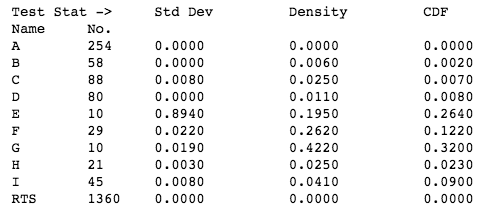
\includegraphics[width=0.8\linewidth]{images/mid_ratio_perm.png}
\caption{Results for Permutation Tests for Mid Ratios}
\label{mid_ratio_perm}
\end{figure}

\subsubsection{Limitations of Permutation Tests} % (fold)
\label{ssub:limitations_of_permutation_test}

% subsubsection limitations_of_permutation_test (end)
The main concern we have for the set up of the permutation tests we discussed is the huge fraction of the data
collected by RTS. 
The $p$-values indicate the chance of the difference
between the two groups (treatment and control), so a low $p$-value means
that the treatment group is likely to be different than the control
group. 
Here, however, the control group (RTS) has a dominant effect, hence the conclusion that the data of the
other lab members are very different from the data of RTS. 

To draw more accurate conclusions about the other researchers, we performed additional permutation tests excluding data provided by RTS, illustrated in Figure~\ref{fig:perm_2}.
This approach has a bias, because almost 2/3rd of the data are ignored, but it allows to give some answers which were consistent with the authors' expectations-- there is some statistical evidence that the others did not fabricated data.

\begin{figure}[htbp]
\label{fig:perm_2}
\centering
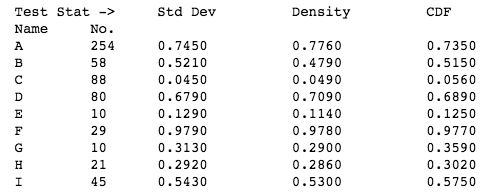
\includegraphics[width=0.8\linewidth]{images/mid_ratio_perm_no_rts.png}
\caption{Results for Permutation Tests without RTS  for Mid Ratios}
\end{figure}

    \subsection{Additional Tests for Digit
Analysis}\label{additional-tests-for-digit-analysis}

For the terminal digit and equal digits tests, we extended the tests in the paper by running the additional experiments: 
\begin{itemize}
    \item chi-square test for goodness of fit for terminal digit analysis,
for each of the lab members and outside labs;
    \item chi-square test for goodness of fit for equal digits analysis, for each of the lab members and outside labs;
    \item permutation tests for terminal digit analysis considering RTS and the other investigators.
 \end{itemize}

    \subsubsection{Chi-square test Tests for Terminal Digit
Analysis}\label{chi-square-test-tests-for-terminal-digit-analysis}

To understand how single investigators contributions are distributed
with respect to RTS and the outside labs, we decided to analyze data
from all the other investigators individually. To do so, we
performed a chi-square test for goodness of fit for each of them. The
following tables summarized our results:

\begin{figure}[H]
\label{fig:chi-sum}
\centering
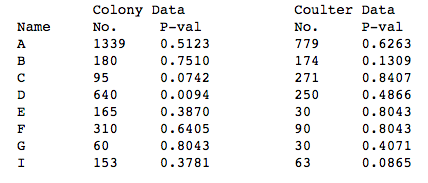
\includegraphics[width=0.7\linewidth]{images/raaz_term_chi_summary.png}
\caption{Chi Square Tests for Terminal Digits in Coulter and colony
Counts}
\end{figure}

Reading the table in Figure~\ref{fig:chi-sum}, one can notice that the $p$-value for D, for Coulter Data is $<1\%$, while all the other $p$-values are well above $1\%$.

    \subsubsection{Chi-square test Tests for Equal Digits
Analysis}\label{chi-square-test-tests-for-equal-digits-analysis}

Also for the Equal Digits Analysis we performed the chi-square test for
goodness of fit using the data of the individual investigators in the
lab, in a setting similar to the previous test.
\begin{figure}[H]
\centering
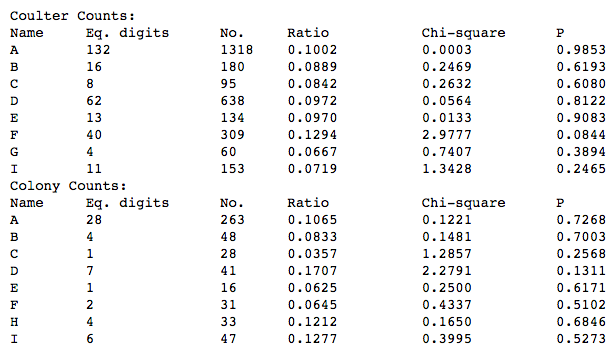
\includegraphics[width=0.9\linewidth]{images/raaz_eq_chi_elaborate.png}
\caption{Chi Square Tests for Equal Terminal Pair in Coulter and Colony
Counts}
\end{figure}

Here none of the $p$-values look abnormally low. One can argue that for $A$ it is very high but, according to the practice of deciding thresholds before seeing the results, none of the results are surprising.

    \subsubsection{Permutation Test for Terminal Digit
Analysis}\label{permutation-test-for-terminal-digit-analysis}

The following tables illustrate the permutation test results using the
same test statistics as for mid-ratios:

\begin{figure}[H]
\centering
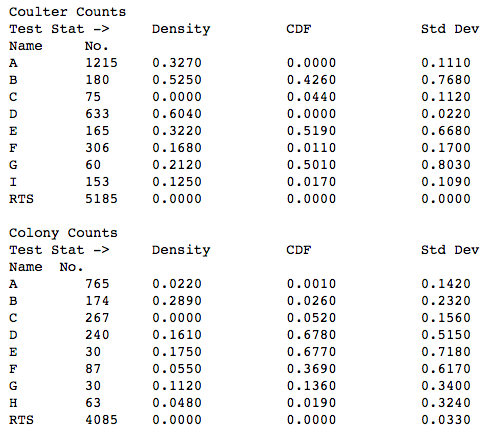
\includegraphics[width=0.7\linewidth]{images/raaz_eq_perm_summary.png}
\caption{Permutation Tests for Terminal Digit Analysis, Coulter counts}
\end{figure}

In all the above cases, it is possible to see how RTS data is
consistently suspicious, which is a confirmation of the authors'
suspects. And, as pointed before, the huge fraction of data collected
by RTS contributes towards the low $p$-values for other individual
researchers as well. 
We performed also permutation tests excluding RTS data
and got better $p$-values (similarly to the previous experiment). 
For sake of brevity, we avoid mentioning the
values here.

    \section{Conclusion}\label{conclusion}

    Data fraud is an extremely critical issue in science, engineering and
many other fields. Methods to detect manipulated data are needed to
identify fraudulent research behaviors. Detecting frauds, however, is a
delicate matter. Challenging the credibility of a researcher or of a
scientific work, in fact, can have heavy consequences for all the parties
involved in the process. Methodologies and techniques used in this kind
of work need to be clear and widely accepted, and they need to produce
results which leave minimal (ideally no) space to ambiguity. Independently, reproducibility of
results is a fundamental element to rule out any doubts that could arise
at any time.

In our review, we carefully analyzed the authors' results
and conclusions by: reproducing all the results that have been
discussed in the paper and proposing and implementing additional tests to
clarify doubts and suggesting additional possibilities to the authors.

We found out that authors' results are correct, although it has not been
possible to reproduce exactly all the experiments due to lack of some
key pieces of information (for instance how data has been
pre-processed). Moreover, we encourage the use of stronger tools like permutation tests and our demonstration can be considered as a promotion of the same. Such tests help the analysis to get \textit{rid of assumptions}, thereby shifting the focus from debate on assumptions to actual anomalies present and to better understanding of individual
investigator's data (besides the RTS) as to how do they compare to the general data pool.

At the end of our review, we do believe that there is a significant evidence that RTS has suspicious data, but we suggest the authors to collect additional material and investigate more, since some of our tests suggest that other investigator's
data have anomalies as well if we do not discount the huge fraction of data given by RTS.

\section*{Acknowledgments} % (fold)
\label{sec:acknowledgments}

We would like to thank the authors H. Pitt and H. Hill for publishing in an open journal, and making the data available for everyone. Also, we would like to thank Prof Philip Stark for his valuable and critical guidelines and timely feedback. We would also like to thank Yuansi Chen for valuable tips with python. As a final note, we would like to claim complete responsibility for all the opinions expressed in this paper.

% section acknowledgments (end)


\bibliographystyle{apalike}
\bibliography{biblio}

    \end{document}
